\section{Requirements and System Model}\label{sec:requirements}
Big data is highly dependent on cloud-edge computing, which makes extensive use of multitenancy.
Mul\-ti-te\-nan\-cy permits sharing one instance of infrastructures, platforms or applications by multiple tenants to optimize costs.
This leads to common scenarios where a service provider offers subscription-based analytics capabilities in the cloud,
or a single data lake is accessed by multiple customers.
Thus, it is a common situation to have a big data pipeline where data and services belong to various organizations,
posing a serious risk of potential privacy and security violation.
In the following of this section,
we present our system model (Section \ref{sec:systemmodel}),
the requirements driving our work (Section \ref{sec:accesscontrol_req}),
and our reference scenario (Section \ref{sec:reference}).

\subsection{System Model}\label{sec:systemmodel}
\AJ{Our system model aims to achieve an optimal service composition to ensure privacy and data quality.
  Within this context, we contemplate an interconnected sequence of services, establishing a pipeline where individual nodes signify distinct services.
  Each stage within the pipeline undertakes the task of data transformation or processing, with the resulting output serving as the input for the subsequent service.
  This model encapsulates what we refer to as a template, visually presented in Figure \ref{fig:service_composition_template}.
  In order to instantiate the template, the selection of services to be executed at each step of the pipeline becomes imperative. At each step, there exists a collection of functionally equivalent services that differ in terms of annotation and data transformation.
  These services are annotated with a set of requirements, such as the owner's information, among others. The annotations play a pivotal role in the creation of policies that determine the eligibility of a service for deployment. For instance, a policy may restrict the usage of services to a specific owner within a particular dataflow. By enforcing such policies, the set of candidate services for a given step is significantly reduced.
  The remaining services undergo evaluation based on their potential impact on the data transformation process. Preference is given to the service that maximizes data quality while ensuring an equal level of data privacy. This evaluation process aids in identifying the most suitable service for a particular step in the pipeline.
  Upon the selection of the most appropriate service for each step, the instantiation of the pipeline is deemed complete. Consequently, the pipeline becomes ready for execution, with the assurance that the chosen services align with the specified requirements and optimize the desired outcomes.
}




Our system is a coalition of organizations that collaboratively execute a Big Data pipeline where
\emph{i)} organizations join without necessarily integrating their cloud-based or on-premises ICT infrastructures,
\emph{ii)} collaborative processes are carried out involving multi-party data collection and analytics,
\emph{iii)} the pipeline can be executed in a centralized or distributed deployment.

It includes 4 different parties:
\emph{i)} the pipeline owners, executing Big Data analytics pipelines,
\emph{ii)} the organizations, providing the different services composing a big data pipeline,
\emph{iii)} the coalitions, as an orchestration of organizations providing all services at the basis of the Big Data analytics pipelines.

A big data pipeline can be defined as a composition of services, each one implementing a job, which can be parallelized to exploit the big data infrastructure capabilities.
It defines executable processes that consist of a set of jobs combined using different structures to form a coherent system.
Depending on the scope, jobs can be roughly classified as
  {\em i)}~\emph{ingestion jobs}, capturing and transforming data with the scope of saving it for further analysis, dealing with different data format (i.e., structured, unstructured, and semi-structured),
{\em ii)}~\emph{analytics jobs}, executing specific analysis on data, which may include data preparation tasks (e.g., normalization, cleaning, selections) to make data suitable for specific analytics,
{\em iii)~visualization jobs}, presenting the output of an analytics to users.

We formally model a Big Data analytics pipeline as follows.

\begin{definition}[Big Data Analytics Pipeline] \label{def:pipeline}
  A Big Data Analytics pipeline \G(\V,\E) is a direct acyclic graph having a root \vi{r}$\in$\V, a vertex \vi{i}$\in$\V$_I$$\subseteq$\V\ for each job \job{i} invocation, two additional vertices \vi{c},\vi{m}$\in$\V$_{\otimes}$$\subset$\V\ for each alternative ($\otimes$) structure modeling the alternative execution (\emph{choice}) of operations and the retrieval (\emph{merge}) of the results, respectively, and two additional vertices \vi{f},\vi{j}$\in$\V$_{\oplus}$$\subset$\V\ for each parallel ($\oplus$) structure modeling the contemporary execution (\emph{fork}) of operations and the integration (\emph{join}) of their results, respectively.
\end{definition}

We note that each vertex \vi{i} model a job \job{i} provided by an organization \org{i}.
We also note that an analytics pipeline can be deployed following a centralized or a decentralized approach as discussed in detail in Section \ref{sec:architecture}.

\begin{figure}[!t]
  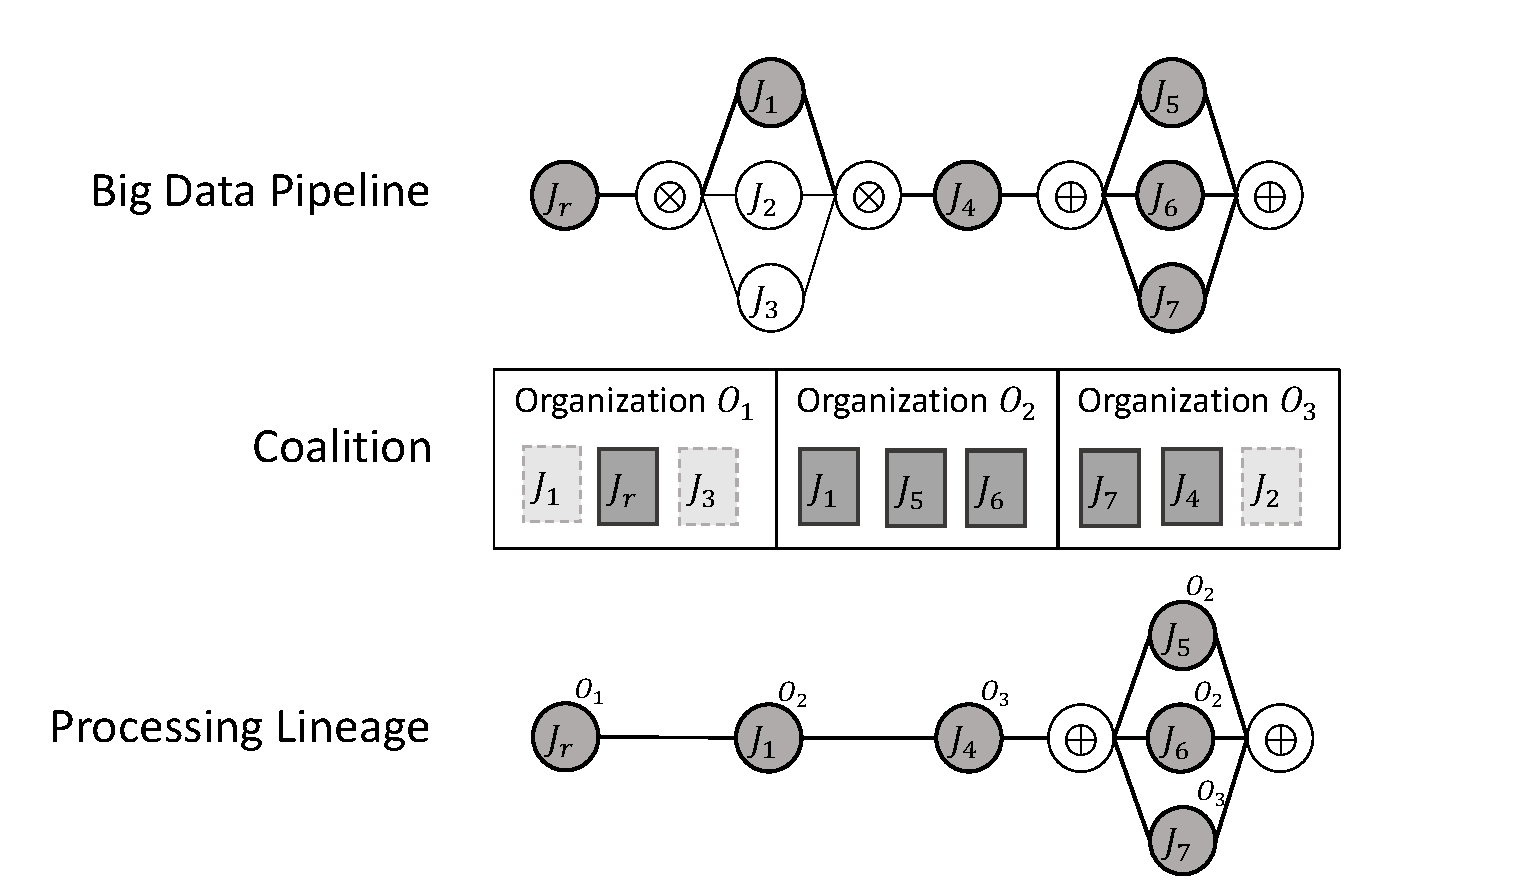
\includegraphics[width=0.98\columnwidth]{generaleFig1.pdf}
  \caption{Big Data Analytics pipeline graphs with a coalition of organization for a given processing lineage.}\label{fig:BDpipeline}
\end{figure}

Figure~\ref{fig:BDpipeline} shows an overview of our system model.
In our model, organizations form coalitions, that is, collaborative networks of autonomous domains implementing a processing lineage of a given a Big Data analytics pipeline where resource sharing is achieved by the distribution of access permissions to coalition members based on negotiated resource-sharing agreements.
A big Data pipeline can be constitute of a set of linear independent path (processing lineage) each of them implemented by coalition. In most cases, these coalitions are dynamic in nature, as changing conditions and trust relationships result in new missions and modifications to coalition membership.
This scenario introduces a clear IT governance conflict: data should be compartmentalized to ensure strong protection, on one side, and shared to enable advanced analytics and key inter-organizational business processes, on the other side.
This results in a set of strict requirements on existing access control systems that are discussed in the following section.

%Solid arrows present the typical batch or analytics model generation flows. Dashed arrows present typical streaming or prediction flows. \CH{togliere dalla figura la linea che separa le due procedure e le scritte ingestion procedure e analytics procedure?}
%The coalition creation is driven by missions including emergency and disaster management, humanitarian operations, or simply interdependent organizations.
%\CH{Qui ho introdotto solo il termine coalition, va spiegato anche il termine federation?}


\section{Policy}
\subsection{Annotations}
\subsection{Transformation}
\subsection{Policy}